\subsection{Vector subspaces of finite dimension}

THEOREM 2. --- Every Hausdorff topological vector space E, of finite dimension n, over a complete non-discrete valued division ring K, is isomorphic to \(K_{s}^{n}\) ; in fact, for every basis \((e_{i})_{1\leqslant i\leqslant n}\) of E on K, the linear mapping \((\xi_{i})\mapsto\sum_{i=1}^{n}\xi_{i}e_{i}\) is an isomorphism of \(K_{s}^{n}\) on E.

Proposition 2 of I, p.~12, implies that th. 2 is true for \(n = 1\) ; we argue by induction on \(n\) . Let \(H\) be the vector subspace of \(E\) generated by \(e_1, e_2, ..., e_{n-1}\) ; the induction hypothesis is that the mapping \((\xi_i)_{1 \leqslant i \leqslant n-1} \mapsto \sum_{i=1}^{n-1} \xi_i e_i\) is an isomorphism of \(K_s^{n-1}\) on \(H\) . The subspace \(H\) , being isomorphic to a product of complete spaces, is complete (GT, II, § 3.5, prop. 10); hence it is closed in \(E\) (GT, II, § 3.4, prop. 8). Let \(D\) be the subspace \(K e_n\) complementary to \(H\) in \(E\) ; \(E\) is the topological direct sum of \(H\) and \(D(I, p. 13, cor. 2)\) , therefore the mapping

\[
\left(\xi_ {i}\right) _ {1 \leqslant i \leqslant n} \mapsto \sum_ {i = 1} ^ {n} \xi_ {i} e _ {i}
\]

of \(\mathbf{K}_s^{n - 1}\times \mathbf{K}_s\) on E is an isomorphism.

When n \textgreater{} 1 the hypothesis that K is complete is essential for the validity of theorem 2. In fact, let K be a non-complete valued division ring, and let \(\hat{K}\) be its completion: for each \(a \neq 0\) of \(\hat{K}\) the set K.a is everywhere dense in \(\hat{K}\) , since \(x \mapsto xa\) is a homeomorphism of \(\hat{K}\) on itself. If \(a \notin K\) , the subspace \(K + Ka\) of the topological vector space \(\hat{K}\) on K is of dimension 2 on K, but it is not isomorphic to \(K_{s}^{2}\) since every subspace of dimension 1 in \(K + Ka\) is dense in \(K + Ka\) .

COROLLARY 1. --- In a Hausdorff topological vector space E over a complete non-discrete valued division ring K, every vector subspace F of finite dimension is closed in E.

For, if \(\mathbf{F}\) is of dimension \(n\) then it is isomorphic to \(\mathbf{K}_s^n\) ; it is therefore complete and hence closed in \(\mathbf{E}\) (GT, II, § 3.4, prop. 8).

COROLLARY 2. --- Let K be a complete non-discrete valued division ring, and E be a Hausdorff topological vector space of finite dimension over K. If F is any topological vector space over K, then every linear mapping of E in F is continuous.

COROLLARY 3. --- In a Hausdorff topological vector space E, over a complete non-discrete valued division ring, every finite independent set is topologically independent.

COROLLARY 4. --- Let E be a topological vector space over a complete non-discrete valued division ring. If M is a closed vector subspace of E and F is a vector subspace of E of finite dimension, then the subspace \(M + F\) is closed in E.

Write \(\phi\) for the canonical homomorphism of \(E\) on the quotient space \(E / M\) (necessarily Hausdorff). Then the subspace \(M + F\) is identical with \(\bar{\phi}^{1}(\phi(F))\) . Now \(\phi(F)\) is of finite dimension in \(E / M\) , therefore (cor. 1) \(\phi(F)\) is closed in \(E / M\) , and, in consequence, \(\bar{\phi}^{1}(\phi(F))\) is closed in \(E\) .

\pandocbounded{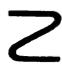
\includegraphics[keepaspectratio]{images/part001_c7194320.jpg}}

We note that, if M and N are any two closed vector subspaces in a Hausdorff topological vector space E, then \(M + N\) is not necessarily closed in E, * even if E is a Hilbert space * (cf.~IV, p.~64, exerc. 13, d)).

PROPOSITION 3. --- Let E be a topological vector space over a complete non-discrete valued division ring K. Let M be a closed vector subspace of finite codimension n in E. Then every subspace N that is an algebraic complement of M in E is also a topological complement.

In N, the set \(\{0\}\) is closed, since it is the intersection of N and the set M which is closed in E; thus N is Hausdorff. As E/M is also Hausdorff, the canonical mapping of N on E/M, which is linear and bijective, is bicontinuous (I, p.~14, cor. 2), from which the proposition follows.

COROLLARY. --- Let E and F be two topological vector spaces over a complete non-discrete valued division ring. If F is Hausdorff and of finite dimension, then every continuous linear mapping of E on F is a strict morphism.

Remark. --- The results of Nos 2, 3 are no longer valid when K is discrete. For example, let \(K_{1}\) be a non-discrete valued division ring and K be the discrete division ring obtained by endowing \(K_{1}\) with the improper absolute value on \(K_{1}\) . Then \(K_{1}\) is a topological vector space of dimension 1 over K, but it is not isomorphic to \(K_{s}\) . However, we can show that the results of Nos 2, 3 are valid even when K is discrete, provided that we impose on the topological vector spaces considered, the property of having a fundamental system of balanced neighbourhoods of 0 (i.e.~neighbourhoods V such that \(K.V = V\) ) (I, p.~27, exerc. 14); this condition (which is always satisfied when K is a non-discrete valued division ring cf.~I, p.~7, prop. 4) is not valid for all topological vector spaces over K as the preceding example shows.

